
\chapter{Detecting and injecting binaries}


In this chapter, we introduce a new algorithm to detect and record binary system in nbody simulations. With this tool, we analyse the spontaneous binary population arising in the \HubLem systems and we describe a binary injection method to complete this population to match the observations.




\section{A new binary detection algorithm}


\subsection{Density comparison}

The study of binary populations in nbody simulations requires an algorithm to detect binary systems and compute their characteristics. The simplest approach is to compute all star-star energies and consider bound pairs as binaries. This records a lot of ephemeral interactions, as n-body dynamics cause transient bound systems. An additional criteria is needed to assess the stability and robustness of a pair as a binary.

\begin{figure}
\begin{center}
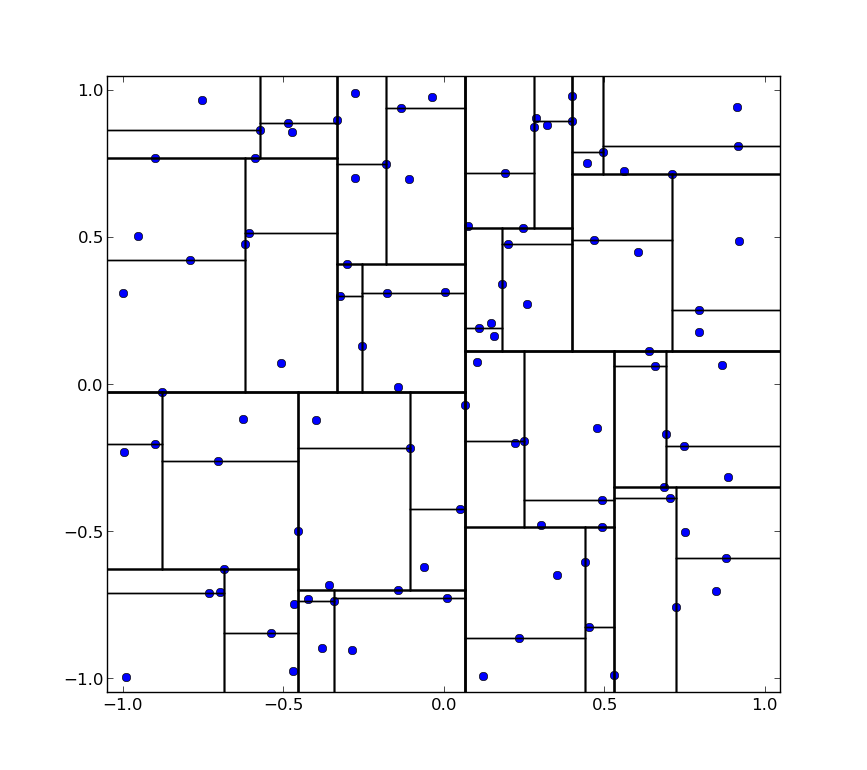
\includegraphics[width=0.6\textwidth]{Figures/5_kdtree}
\caption{Illustration of a kdtree for a random two-dimensional distribution (blue dots).}
\label{Fig:5_kdtree}
\end{center}
\end{figure}


We introduce a new algorithm based on the idea of a density threshold: binaries must be denser than their direct environment. Before describing the algorithm, we wish to emphasize the importance of neighbour searches in this kind of study. Be it to obtain bound pairs or to study said pair direct environment, the quick retrieval of neighbours is crucial to an effective algorithm.

The method described here relies on the KD-tree algorithm \citep{numericalrecipes}. While brute-force neighbour searches scale as $\propto N$, as all stars in the system have to be checked as potential neighbours, a KD tree, once built, performs neighbour searches with algorithmic complexity $\propto\log (N)$. The tree is built by sorting particles along one dimension, splitting them at the median, then sorting each branch along another dimension, splitting them again, and so on, cycling over dimensions. A two-dimensionnal example is show on Fig~\ref{Fig:5_kdtree}.





First, binary candidates are identified as negative energy pairs. The semi-major axis of the system is derived from the star motions, then a "binary density" is computed, with $a$ the binary's semi-major axis :
\begin{equation}
 \rho_{binary} = \frac{m_1 + m_2 }{4\pi a^3/3 }\, .
\end{equation}
This is then compared to the local neighbour density, defined as the cumulated mass of a fixed number $N_{nb}$ of neighbours to the pair over the spherical volume reaching to the last neighbour.
\begin{equation}
 \rho_{local} =  \frac{\sum\limits_{i=0}^{N_{nb}} m_i}{ 4 \pi r_{N_{nb}}^3 /3} .
\end{equation}


\begin{figure}
\begin{center}
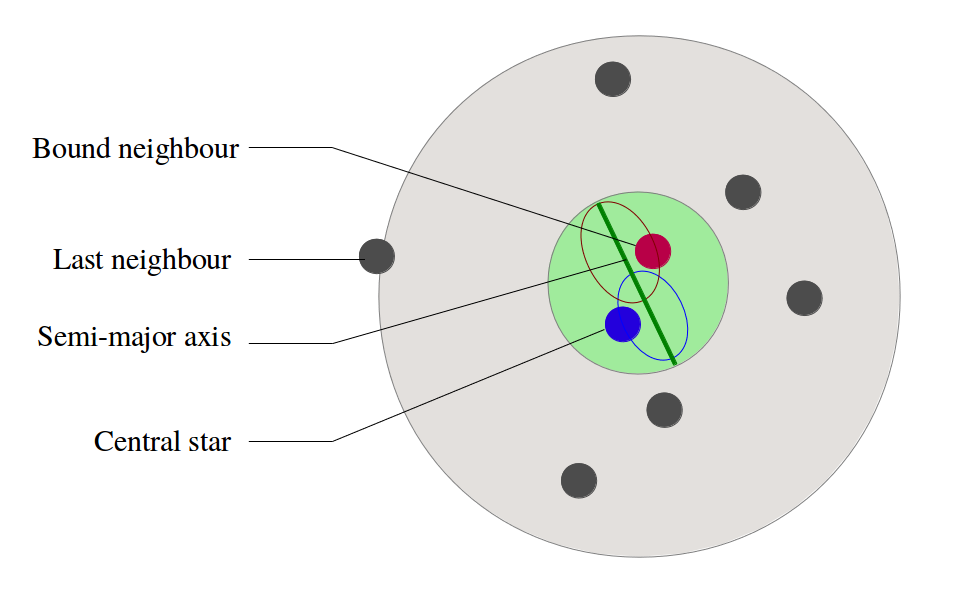
\includegraphics[width=0.6\textwidth]{Figures/5_neighbours}
\caption{Illustration of the density threshold method. The central blue stars and the red bound neighbour describe a two-body orbit shown on the figure while the green bar indicates the major-axis of the system. This defines the binary density, green sphere, while the local density is defined with the grey stars, the other neighbours. Here, $N_{nb}$ was set to 7. }
\label{Fig:5_neighbours}
\end{center}
\end{figure}




If the density ratio exceeds a threshold $D$, 
\begin{equation}
\label{Eq:density_ratio}
\frac{ \rho_{binary} }{ \rho_{local} } > D,
\end{equation}
the pair is registered as a binary.  Other authors, eg \cite{Parker2009,Lomax2015}, have used close hybrids of the criteria that we have implemented.

Stars can be found to be part of several binaries at once, which happens more often for massive stars as they clear more easily the density threshold. When that happens, the algorithm selects from such connected systems only the pairs exhibiting the lowest (most negative) binding energy.

This method has two free parameters: $N_{nb}$ and $D$. $N_{nb}$ can be set from 6 to 10 neighbours without a substantial impact on the detection. The density ratio is a more critical parameter, as if it is chosen too low, a lot of ephemeral binaries are found, while a high value picks only the closest binaries, ignoring wider, yet stable, systems.



\subsection{Choosing a density ratio}



\begin{figure}
\begin{center}
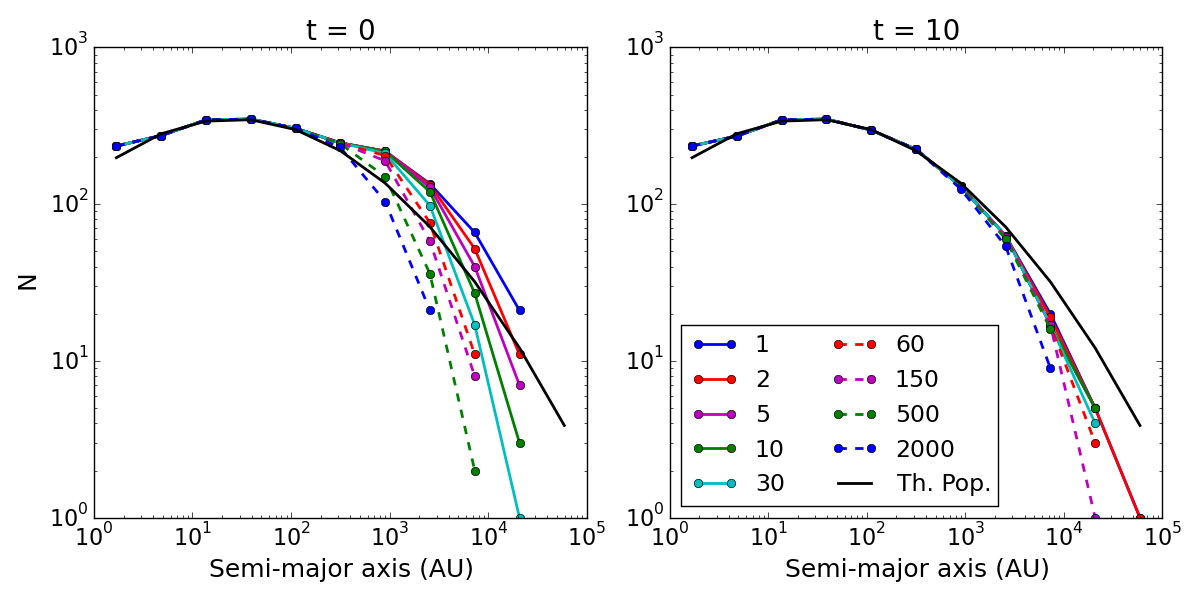
\includegraphics[width=\textwidth]{Figures/5_sm_ratios}
\caption{Semi-major axis histograms for various value of the density ratio $D$ at t=0 and 10 H.u for a 10k star King model and a binary fraction $f_b =0.3$. The injected log-normal population is shown as a black solid line.}
\label{Fig:5_sm_ratios}
\end{center}
\end{figure}



We wish to find a good compromise value for the critical density ratio $D$ that maximizes the number of detected stable binaries without collecting too much transient system. To do so, we explore the results brought by different values of $D$ in a nbody system containing binaries.

We create a virialized King model with N = 10000 stars and a binary fraction of 0.3. This means there are 2300 binaries and 5400 single stars:
\begin{equation}
f_b = \frac{N_b}{N_s + N_b} = \frac{N_b}{N-N_b} \quad \implies \quad N_b = \frac{f_b}{1+f_b} N = 2300.
\end{equation}
The binaries follow the \cite{Raghavan2010} log-normal distribution introduced in \ref{Sec:0_raghavan}. We let the system run for 10 H.u, or 12 crossing times, and write a snapshot every 0.1 H.u.

The binary detection is ran over all snapshots once per density ratio in the following list:

\begin{center}
\begin{tabular}{l|rrrrrrrrr}
\centering
D  &  2000 & 500 & 150 & 60 & 30 & 10 & 5 & 2 & 1\\ 
\end{tabular}
\end{center}

We show on Fig~\ref{Fig:5_sm_ratios} the semi-major axis distribution retrieved for various $D$ for t=0 and t=10, with the theoretical injected population as a solid black line.



\begin{figure}
\begin{center}
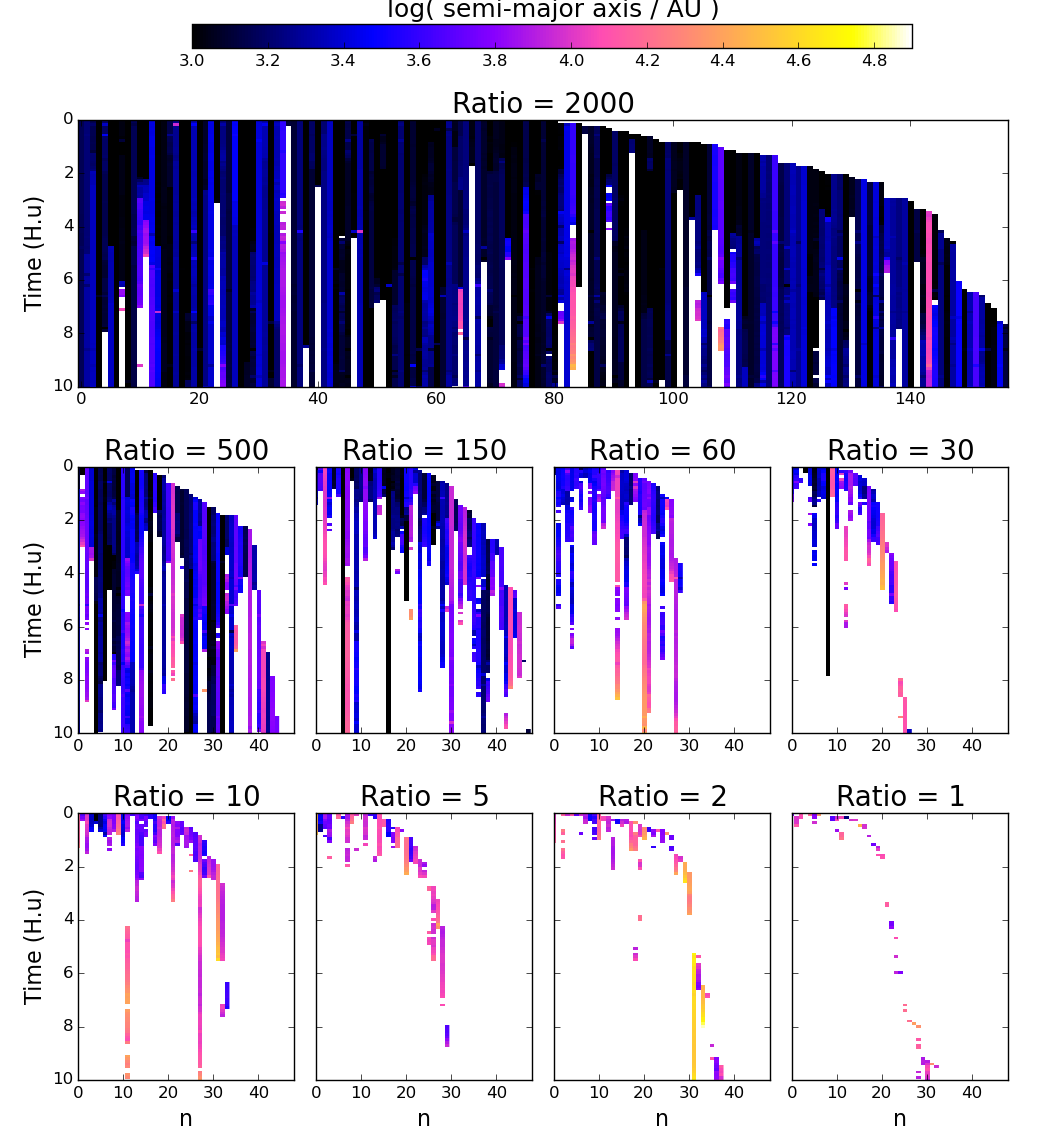
\includegraphics[width=0.9\textwidth]{Figures/5_flickering}
\caption{Visualization of the wide ($a>1000$ AU) binary population in a King model over time. Large upper panel show the evolution of all binaries detected for a density ratio $D=2000$, ordered by time of first detection. Each lower sub-panel show the new binaries detected with the new, lower, value of $D$ compared to the previous one.}
\label{Fig:5_flickering}
\end{center}
\end{figure}

Looking at the left panel, for t=0, we see all density ratios return the same population for $a < 1000$ AU, while for higher separation, there are large variations. $D = 2000$ does not detect semi-major axis larger than 3000 AU, while $D = 1$ detects $\sim$ 30 systems with $a > 10^4$ AU. After 12 crossing times, on right panels, we see the tight detected population didn't change, while all wide populations converged. The highest ratios did not undergo much change, while low ratios saw a large depletion of the population they initially returned. 

 We can say that a very high ratio only detect binaries that are garanteed to resist the dynamical processing and survive, while low ratios detect more fragile systems. How ephemeral are these latter binaries ? To evaluate the different population detected by different ratios, we show on Fig~\ref{Fig:5_flickering} the detailed evolution of the wide, $a>1000$ AU population. The large upper panel show all wide binaries evolution (time on y-axis) for $D=2000$, arranged on the x-axis by time of first detection. Each pixel column represents a binary. The smaller sub panels show, for each density ratio, the history of the binaries this ratio detected that the previous, greater ratio did not. A binary that is detected with $D=2000$ will also be detected for $D=500$ and any other lower value. Fig~\ref{Fig:5_flickering} shows what kind of binaries lowering the ratio progressively brings to the detected population. The color codes the logarithm of the semi-major axis in AU, white means the binary is not detected.

The $D=2000$ population is mainly made of stable, relatively tight binaries. About half the binaries are detected at t=0, while the others dynamically form in the system. Some are destroyed, other widened through interactions as their color bars transitions to a lighter color, sometimes after a "flickering" phase, when the detection goes on and off over successive snapshots. This is due to the binary entering a dynamical interaction with a third star or other binary, making the neighbour density undergoing spikes. This interaction leaves the binary with a weaker bound, thus higher binding energy. 

Looking at the populations brought by lower ratios, we see they are progressively wider and more transient/flickering as the ratio lowers, which is to be expected. $D=1$ only brings very ephemeral pairs, often not lasting more than a single snapshot. All ratios bring their share of transient binaries, but $D=10$ is the last to capture relevant, relatively long-lived pairs.

Extreme values of density ratios bring a large difference in the detection of large binaries, but a moderate value like $D=10$ appears the best compromise to capture the substance of a binary population.




